

% Add this line at the top of your document preamble (before \begin{document}):
% \usepackage{subcaption}

\begin{enumerate}
    \item Die PCB mit dem Coupled-Line-Filter wird mit dem Fieldfox an beiden Ausgängen angeschlossen, 
    woraufhin die S-Parameter dessen im Network-Analyzer-Modus vermessen werden. Folgende Leistungsspektren kommt zustande:
    \begin{figure}[H]
        
        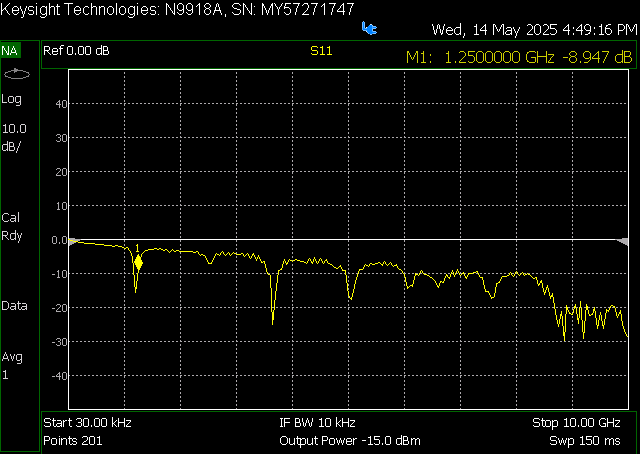
\includegraphics[height=6cm]{Pictures/S11neuCooleGrupp.png}
        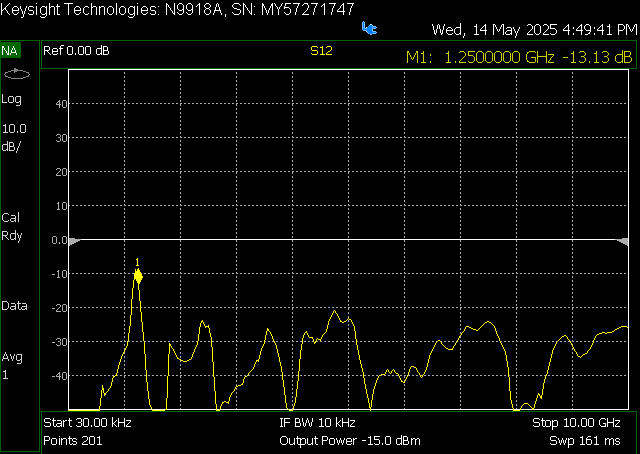
\includegraphics[height=6cm]{Pictures/S12neuCooleGrupp.png}
        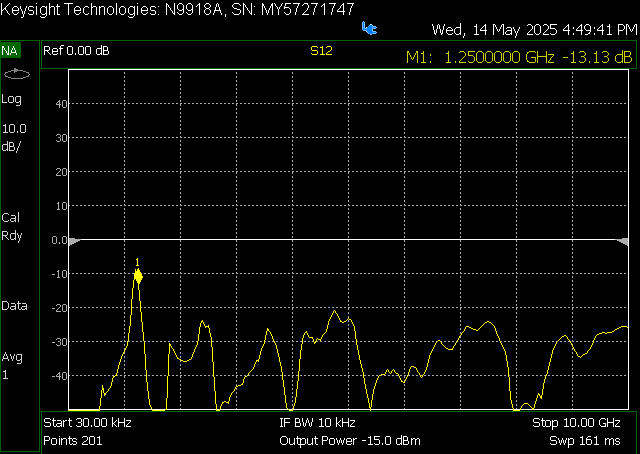
\includegraphics[height=6cm]{Pictures/S12neuCooleGrupp.png}
        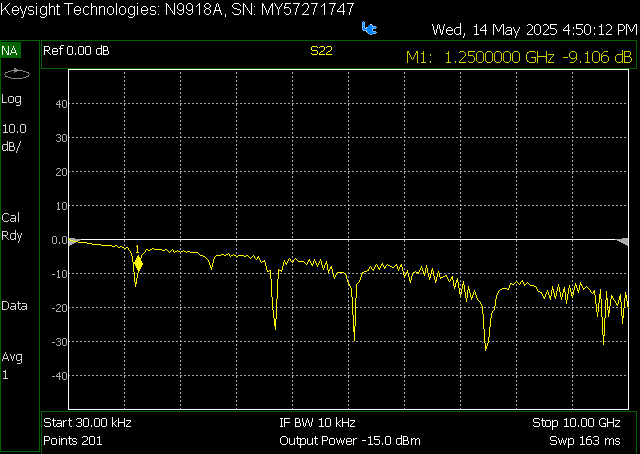
\includegraphics[height=6cm]{Pictures/S22neuCooleGruppe.png}
        \caption{Gemessene S-Parameter des Coupled-Line-Filters.}
        \label{fig:fieldfox_s_parameter}
    \end{figure}
    \item Als nächstes wird der Filter von dem Fieldfox abgekoppelt und mit dem Transmitter mittels einer SMA-Verbindung zur Erzeugung eines Signals verbunden. An den Transmitter wird hierbei eine Spannung $V_CO$ von 5~V angelegt.
    Der Transmitter erzeugt ein Signal bei 1,25~GHz, welches durch den Filter geleitet wird.
    \item Der Network Analyzer wurde so konfiguriert, dass er die S-Parameter des Filters misst.
\end{enumerate}
\section{Messung der S-Parameter im NA-Modus}
\section{Anschluss an den Transmitter und Messung im SA-Modus}
\section{Vergleich des gefilterten und ungefilterten Spektrums}
